\documentclass[conference]{IEEEtran}

\usepackage{cite}
\usepackage{amsmath}
\usepackage{booktabs}
\usepackage{graphicx}
\usepackage{color}
\usepackage{soul}

\usepackage{float} % [H] placement for the qualitative figure (formatting only)
\usepackage{url}
\usepackage[hidelinks]{hyperref}
% Float breathing room (formatting only): keep tables/figures from stacking
% back-to-back on dense two-column pages.
\setlength{\floatsep}{10pt plus 2pt minus 2pt}
\setlength{\textfloatsep}{12pt plus 2pt minus 2pt}
\setlength{\intextsep}{10pt plus 2pt minus 2pt}
\hypersetup{
  pdftitle={Source-Domain Accuracy and Zero-Shot Transfer of Nano-Scale YOLO Detectors for Road Damage Detection},
  pdfauthor={Faaris Khairrudin and Gamma Kosala}
}

% DRAFT SWITCHES: change a single \...true to \...false to omit that analysis.
% The source and zero-shot comparison stay in the paper regardless of switches.
\newif\ifsourceexamples     \sourceexamplesfalse    % six-label illustration
\newif\ifdistractoranalysis \distractoranalysistrue % four- vs six-class training
\newif\ifcountryanalysis   \countryanalysistrue  % common-four-class country comparison
\newif\ifcoretransferanalysis \coretransferanalysistrue % four- vs five-class domain contrast
\newif\ifmaterialanalysis  \materialanalysistrue % target GT/prediction case studies
\newif\iffeaturevizanalysis \featurevizanalysistrue % exploratory earlier-export image statistics/embedding

% TODO (submission): confirm author list, affiliation, and email.
% DONE (2026-10-08): verified primary sources now in references.bib
% (tian2025yolov12_primary = arXiv:2502.12524; sapkota2025yolo26_primary = arXiv:2509.25164).
\begin{document}

\title{Source-Domain Accuracy and Zero-Shot Transfer of Nano-Scale YOLO Detectors for Road Damage Detection}

\author{\IEEEauthorblockN{Faaris Khairrudin}
\IEEEauthorblockA{\textit{School of Computing}\\
\textit{Telkom University}\\
Bandung, Indonesia\\
faariskhairrudin@student.telkomuniversity.ac.id}
\and
\IEEEauthorblockN{Gamma Kosala}
\IEEEauthorblockA{\textit{School of Computing}\\
\textit{Telkom University}\\
Bandung, Indonesia\\
gammakosala@telkomuniversity.ac.id}
}

\maketitle

\begin{abstract}
Road-damage detectors must distinguish defects from other road-surface objects while maintaining useful performance outside their training domain. We compared five nano-scale YOLO detectors on the six-class Asian subset of N-RDD2024, comprising four damage classes and two additional surface-object classes. Mean average precision (mAP) at an intersection-over-union (IoU) threshold of 0.5 is the primary metric. We evaluated the six-class models without target-domain fine-tuning on the five annotated classes of an Indonesian road image set. On the 995-image source test set, a local reconstruction of YOLO-RD achieved the highest six-class mAP at IoU 0.5, 0.661; YOLOv12n achieved 0.654. On the 307-image, 502-instance target export, YOLOv12n obtained the highest five-class mAP at IoU 0.5, 0.337, versus 0.618 on the same five classes of the source test set. \ifdistractoranalysis Four-class versus six-class training produced only small, mixed changes in damage-class mAP at IoU 0.5; these results do not establish a benefit from explicitly labeling the two additional classes.\fi{} These single-seed results show that source-domain ranking and zero-shot ranking need not coincide. Target annotation quality control and a standardized throughput protocol remain to be documented before submission.
\end{abstract}

\begin{IEEEkeywords}
road damage detection, YOLO, object detection, domain shift, zero-shot evaluation, class-label ablation
\end{IEEEkeywords}

\section{Introduction}
Road-damage detection can support inspection of cracks and potholes, but image-based detectors encounter variation in pavement appearance and camera conditions. In particular, a detector trained on roads in one set of countries may encounter different surface textures, image viewpoints, and class frequencies on an unseen route. Multi-country road-damage datasets provide a basis for training and evaluating such systems \cite{arya2021deep,Arya2024846}. Manholes and pavement patches can visually resemble potholes, motivating their annotation as separate classes in prior work \cite{matouq2024ai}. N-RDD2024 additionally annotates road-surface objects beyond the four commonly used damage classes \cite{kaya2024nrdd2024}. Whether explicitly learning these additional labels improves detection of the damage classes is an empirical question, not a consequence of their apparent visual similarity.

Recent YOLO-based road-damage methods emphasize either compact computation or richer feature extraction \cite{Li2024,Zeng2024,Wang2025}. Results reported on different datasets and training recipes cannot isolate the relative behavior of these designs. Moreover, a detector selected solely by its source-domain score may perform differently on an unseen target export. We therefore ask how five nano-scale detectors compare on a common six-class source test set and how much performance they retain on an unseen target split without fine-tuning.
% REVIEW-ANALYSIS [covered]: Source-Domain Detection and Computational Trade-off
% and Zero-Shot Target Evaluation answer the comparison above; check final tables.
% REVIEW-ANALYSIS [conditional]: The next question is answered in Four- versus
% Six-Class Training (Table~\ref{tab:ablation}); keep it paired with that section.
\ifdistractoranalysis We also ask what changes when manhole and patchy-road labels are removed from training, measured on the same four damage classes.\fi

This study contributes a comparison under a broadly shared training policy and a class-aligned source--target evaluation. \ifdistractoranalysis It additionally tests the label-set ablation on common damage classes.\fi{} We report observed differences descriptively: the experiments used one documented seed, and the available target metadata do not establish a representative sample of Indonesian roads.

\section{Related Work}
\subsection{Datasets and Cross-Domain Evaluation}
RDD2022 assembled road-damage images across multiple countries and established a common set of crack and pothole labels \cite{Arya2024846}. N-RDD2024 extends the label vocabulary to additional defects and road-surface objects, including manholes and patched roads \cite{kaya2024nrdd2024}. Earlier cross-country road-damage work motivates testing beyond the training distribution \cite{arya2021deep}; however, a performance difference between two differently composed evaluation splits alone cannot identify the physical cause of the difference.

\subsection{Compact Detection Architectures}
YOLO performs object detection in a single-stage framework \cite{redmon2016you}. Road-damage YOLO variants explore attention, lightweight convolutions, and feature-fusion changes, including SimAM/GhostConv and GhostConv/ECA designs \cite{Li2024,Wu2023}. Among the models compared here, YOLOv8-PD combines a bottleneck-transformer block and large-separable-kernel attention with C2fGhost neck blocks and a lightweight shared-convolution head \cite{Zeng2024}, whereas YOLO-RD integrates star-operation backbone blocks, multi-dimensional auxiliary fusion in the neck, and a wavelet-convolution head \cite{Wang2025}.

\section{Materials and Methods}
\subsection{Source and Target Data}
We used the N-RDD2024 Asian subset (China, Japan, and India) with four damage labels: longitudinal crack (D00), transverse crack (D10), alligator crack (D20), and pothole (D40). Of N-RDD2024's ten categories, we retained manhole (D70) and patchy road (D80) alongside the four core damage classes because of their potential visual similarity to potholes \cite{kaya2024nrdd2024,matouq2024ai}. The train, validation, and test splits contained 6,777, 1,898, and 995 images, respectively, with 17,092, 4,773, and 2,425 label instances in the split inventory. \ifdistractoranalysis The corresponding four-class label inventories contained 14,351, 3,996, and 2,035 instances; images were retained when the two additional labels were removed.\fi{} Patchy road had 471 training instances, compared with 4,555 longitudinal-crack instances, a 9.7-fold count difference; manhole had 2,270 training instances. One duplicate validation annotation was removed by the Ultralytics evaluator; the instance counts above describe the dataset inventory rather than the post-scan evaluation count. \ifsourceexamples Fig.~\ref{fig:source-classes} illustrates the six source labels.

\begin{figure*}[!t]
\centering
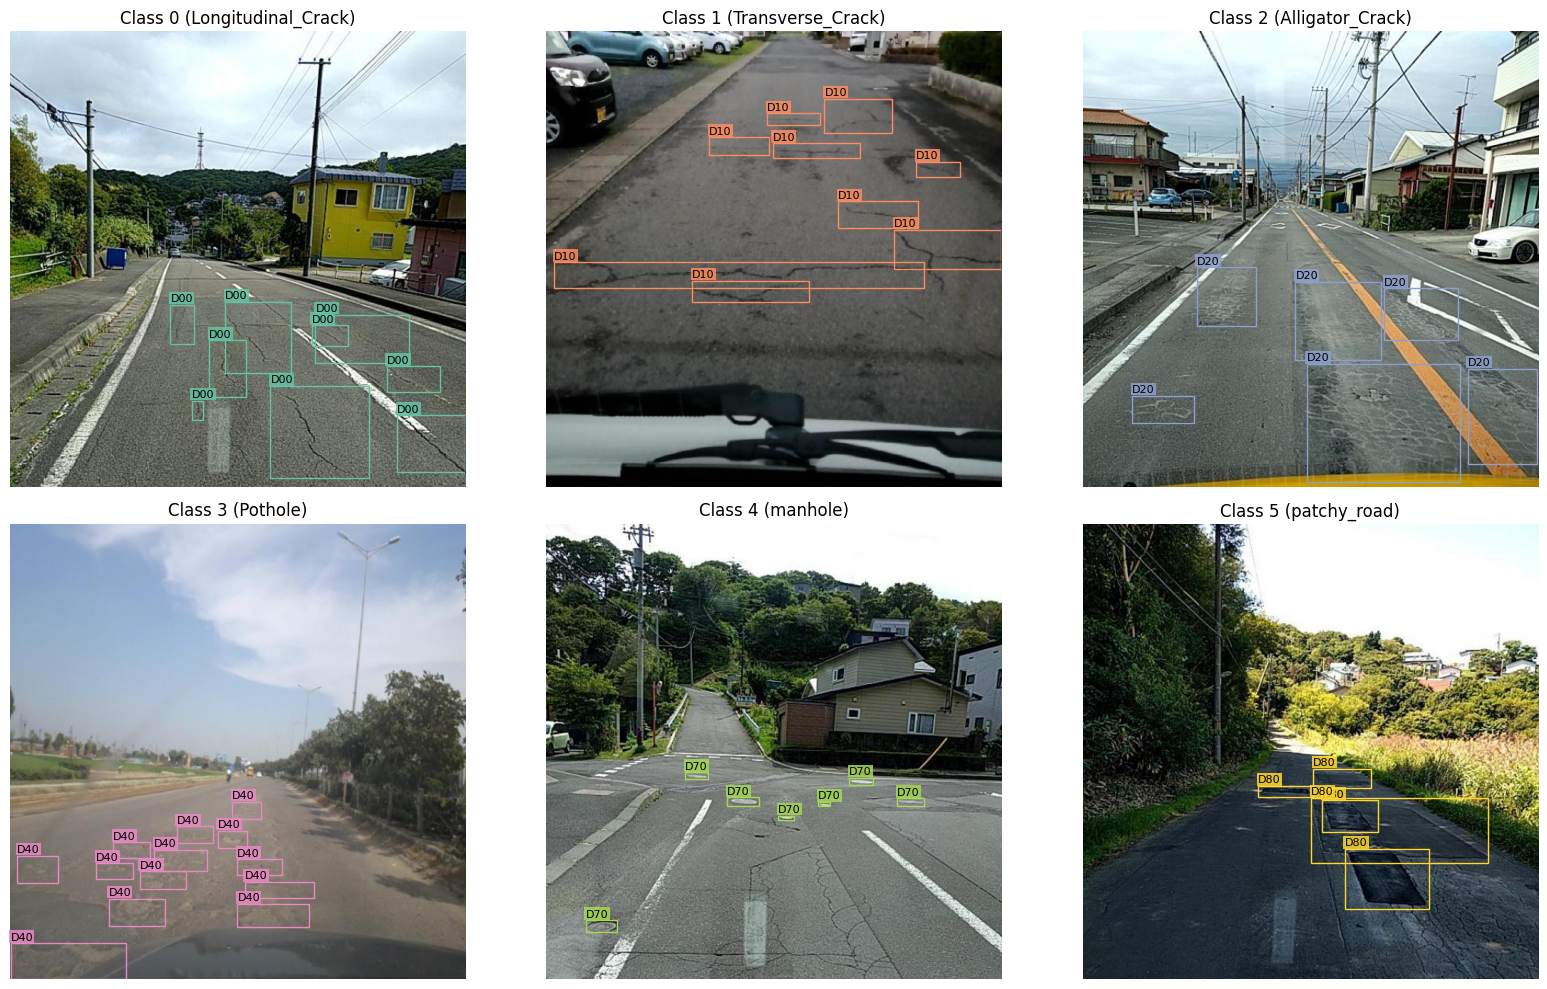
\includegraphics[width=0.83\textwidth]{gambar/class_examples.png}
\caption{Annotated examples of the six source-domain categories: D00, D10, D20, D40, D70, and D80. These are illustrations, not evidence of model-specific errors.}
\label{fig:source-classes}
\end{figure*}
\fi

The target images were collected along Jl. Raya Bojongsoang, Bandung Regency, Indonesia, using a road-facing smartphone video recorded at 1080p. Frames were sampled at 1 frame/s, yielding approximately 1,000 candidate frames for curation and annotation in Roboflow. The analyzed export contains 307 images resized to 640 $\times$ 640, 502 annotated instances, and 39 images with empty labels retained as background examples. Longitudinal crack accounts for 231 target instances; patchy road has only 21. Only the export's \texttt{valid} split was available; we used it for zero-shot evaluation, not training. Five target labels were mapped by class name to the source taxonomy: alligator crack, longitudinal crack, patchy road, pothole, and transverse crack. There was no target ground truth for manhole, so that class was excluded from five-class target aggregates. % REVIEW-METHOD [pending]: archive the exact annotation release and document frame selection criteria, label QC, video-frame dependence, and possible source overlap.

\subsection{Compared Models and Training}
We evaluated YOLOv8n, YOLOv12n \cite{tian2025yolov12_primary}, YOLO26n \cite{sapkota2025yolo26_primary}, and nano-scale Ultralytics reconstructions of YOLOv8-PD and YOLO-RD \cite{Zeng2024,Wang2025}. The reconstructions implement selected design elements rather than bit-exact reproductions of the authors' models. We trained all five six-class models with 640-pixel inputs and seed 42 for up to 300 epochs, using early stopping with patience 40. Shared augmentations were Mosaic (1.0), MixUp (0.05), horizontal flip (0.5), translation (0.10), and scale (0.50); rotation was disabled. To account for unequal training-instance counts across classes, we applied effective-number-derived per-class weights ($\beta=0.999$) to the binary-cross-entropy classification component of the detection loss \cite{cui2019class}.

Batch size and mixed-precision settings varied across models. YOLO26n followed the shared experimental policy, which may differ from its architecture-specific recommended recipe. These factors limit attribution of performance differences solely to architecture.
% REVIEW-METHOD [conditional]: This ablation design is evaluated on the same four
% damage labels in Four- versus Six-Class Training; no YOLO-RD four-class run.
\ifdistractoranalysis For the label-set ablation, four separate four-class models (YOLOv8n, YOLOv12n, YOLO26n, and YOLOv8-PD) were trained after removing D70/D80 annotations. YOLO-RD had no corresponding four-class run.\fi

\subsection{Metrics and Comparison Rules}
We report class-averaged average precision (AP) at IoU 0.5 (mAP@0.5), mAP over IoU thresholds 0.5--0.95, and macro-averaged F1. For the target comparison, we additionally report F1 weighted by ground-truth class support. \ifdistractoranalysis For the ablation, we average per-class AP over \emph{only} D00, D10, D20, and D40 for both training regimes; directly contrasting the six-class and four-class aggregate mAP would change the evaluated label set.\fi{} In the target evaluation, the five annotated classes are compared with the corresponding five-class average recomputed from source test per-class results. We define the descriptive relative difference as
\begin{equation}
\Delta_{\mathrm{rel}} = 100\left(1-\frac{\mathrm{mAP}^{\mathrm{target}}_{5}}{\mathrm{mAP}^{\mathrm{source}}_{5}}\right)\%,
\label{eq:relative-drop}
\end{equation}
where the subscript denotes the five shared labels, not five-class training. Equation~\eqref{eq:relative-drop} is used only for the descriptive source--target contrast in Table~\ref{tab:transfer}\ifcoretransferanalysis{} and Table~\ref{tab:core-transfer}\fi. Source and target evaluations used 640-pixel inputs, confidence threshold 0.001, and non-maximum suppression (NMS) IoU threshold 0.6 where applicable. No target-domain fine-tuning was performed. Because the target class distribution and image selection differ from the source test set, $\Delta_{\mathrm{rel}}$ is a cross-set performance contrast, not a causal estimate of a specific domain factor.

\section{Results and Discussion}
\subsection{Source-Domain Detection and Computational Trade-off}
% REVIEW-METHOD [pending]: FPS is only a recorded throughput proxy; rerun with
% a canonical timing protocol or remove the FPS column before submission.
Table~\ref{tab:source} reports the six-class source test results. YOLO-RD obtained the highest mAP@0.5 (0.661) and macro-F1 (0.633). Its mAP@0.5:0.95 of 0.371 was tied, to three decimal places, with YOLOv12n. YOLO26n had the lowest summary-reported computation (5.2 GFLOPs), while YOLOv8-PD had the lowest parameter count (2.47 M) and the highest recorded throughput estimate. YOLO-RD had the highest mAP@0.5 but also the highest GFLOPs (12.8). These rankings are observations from one run per model, not statistically resolved differences or evidence of intrinsic superiority.

\begin{table*}[!t]
\centering
\caption{Six-class N-RDD2024 source test performance and model complexity (995 images). Complexity values are evaluation-time summaries; FPS is a project-recorded estimate.}
\label{tab:source}
\footnotesize
\setlength{\tabcolsep}{6pt}
\begin{tabular}{lrrrrrr}
\toprule
Model & mAP@0.5 & mAP@0.5:.95 & Macro-F1 & Params (M) & GFLOPs$^{\dagger}$ & FPS$^{*}$ \\
\midrule
YOLOv8n    & 0.648 & 0.364 & 0.617 & 3.01 & 8.1  & 219.7 \\
YOLOv12n   & 0.654 & 0.371 & 0.619 & 2.56 & 6.3  & 319.3 \\
YOLO26n    & 0.625 & 0.358 & 0.606 & 2.38 & 5.2  & 293.3 \\
YOLOv8-PD  & 0.646 & 0.362 & 0.627 & 2.47 & 7.6  & 368.4 \\
YOLO-RD    & \textbf{0.661} & \textbf{0.371} & \textbf{0.633} & 7.09 & 12.8 & 189.4 \\
\bottomrule
\end{tabular}
\par\smallskip
{\scriptsize $^{*}$Project-recorded estimate on a system reporting an NVIDIA RTX 4070 SUPER; timing protocol is unreconciled and this is not an edge-device benchmark. $^{\dagger}$Parameter counts and GFLOPs are from Ultralytics 8.4.108 evaluation-time model summaries at 640-pixel input; GFLOPs are computational estimates, not measured latency.\par}
\end{table*}

Across the five six-class runs, pothole AP@0.5 ranged from 0.526 to 0.541, below the corresponding longitudinal- and alligator-crack values. Manhole AP@0.5 ranged from 0.820 to 0.845, whereas patchy-road AP@0.5 ranged from 0.512 to 0.587 with only 69 test instances. These class-level results do not show that manholes were mislabeled as potholes. The parameter and GFLOP counts summarize model complexity; the FPS values in Table~\ref{tab:source} should not be interpreted as deployment latency or a universal real-time guarantee.

\ifcountryanalysis
\subsection{Country-Labeled Source Subsets}
% REVIEW-ANALYSIS [pending]: Replace rounded country means with exact
% per-country/per-class exports, or omit this optional subsection.
The source test split contained 180 China, 705 Japan, and 110 India images. Direct comparison of their original six-class aggregate AP is misleading: India has just one manhole instance and no patchy-road ground truth. Table~\ref{tab:country-four} instead averages AP@0.5 over the same four damage classes present in all three country-labeled subsets. For YOLOv12n, the approximate scores are 0.933, 0.579, and 0.293, respectively. These arithmetic means are reconstructed from project results-table entries rounded to three decimals; exact per-country per-class exports should replace them before submission.

\begin{table}[!htbp]
\centering
\caption{Approximate source test mAP@0.5 over D00/D10/D20/D40 only, from rounded per-class country results.}
\label{tab:country-four}
\footnotesize
\setlength{\tabcolsep}{5pt}
\begin{tabular}{lrrr}
\toprule
Model & China & Japan & India \\
\midrule
YOLOv8n   & 0.931 & 0.578 & 0.284 \\
YOLOv12n  & 0.933 & 0.579 & 0.293 \\
YOLO26n   & 0.933 & 0.543 & 0.305 \\
YOLOv8-PD & 0.953 & 0.567 & 0.299 \\
YOLO-RD   & 0.945 & 0.587 & 0.304 \\
\bottomrule
\end{tabular}
\end{table}

The common-class ordering was China, Japan, then India for each evaluated model. The Japan training subset contained more images than China's, yet this comparison cannot isolate dataset size from scene composition, viewpoints, or annotation differences. Only 19 transverse-crack instances occurred in the India training subset, making conclusions about this class particularly fragile. Fig.~\ref{fig:country-examples} shows one labeled image and three predictions from each source country; these selected images illustrate differences in detection behavior, not subgroup error frequencies.

\begin{figure*}[!t]
\centering
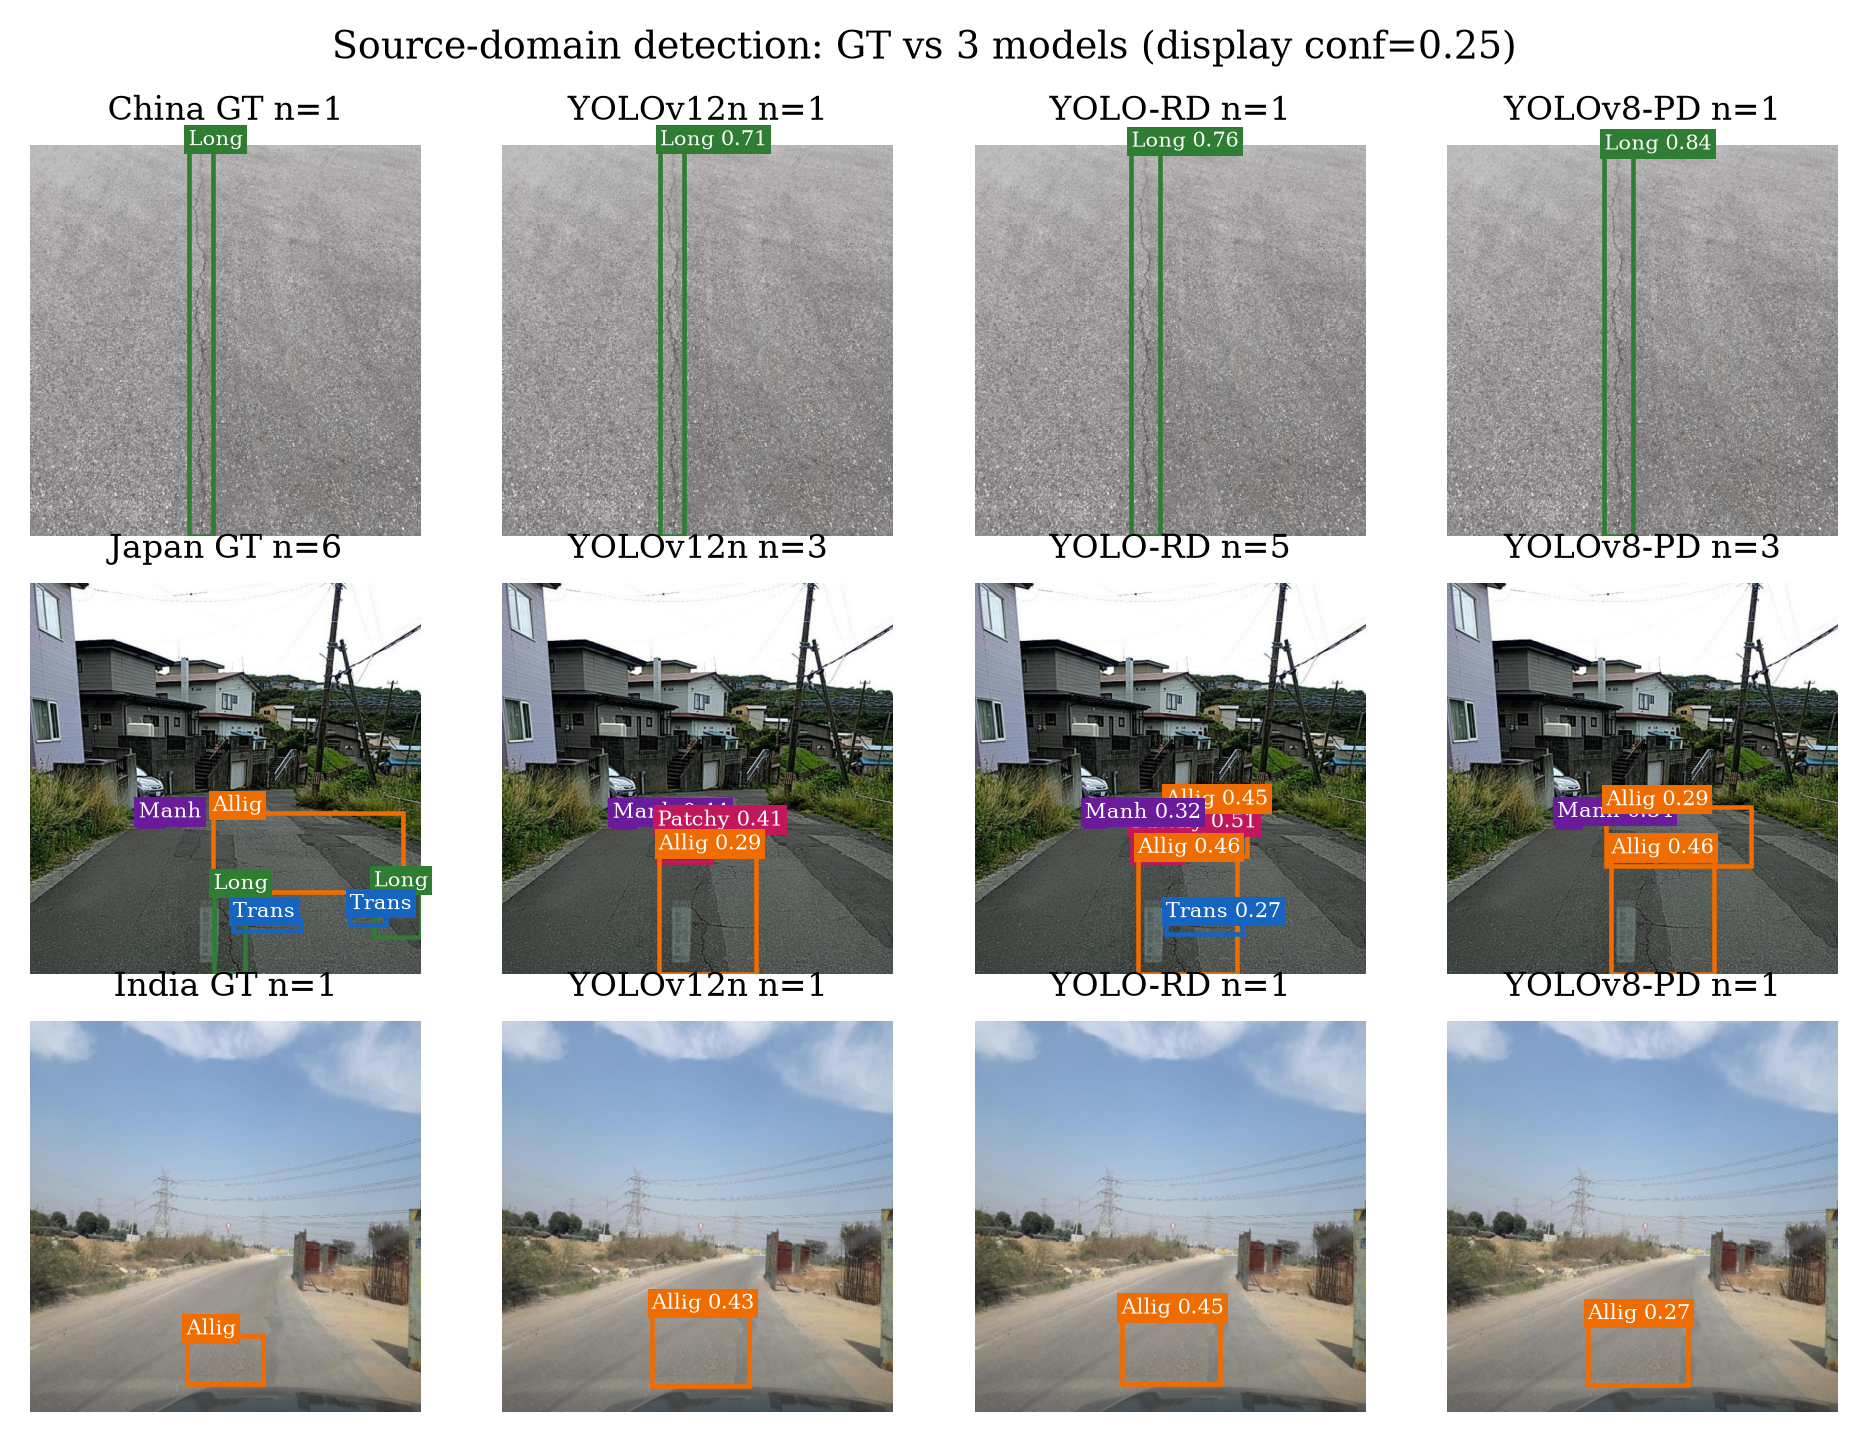
\includegraphics[width=0.86\textwidth]{gambar/paper_fig_country_examples.png}
\caption{Selected source-test examples from China, Japan, and India: ground truth (GT) and predictions from three models at display confidence 0.25. One image per country does not represent its full test split.}
\label{fig:country-examples}
\end{figure*}

Fig.~\ref{fig:domain-examples} compares typical-looking images across the three source subsets and the Indonesian target export. The displayed images were selected near within-subset medians of simple image statistics. They reveal changes in viewpoint, scene content, and pavement appearance, but do not identify which factor accounts for the measured performance differences.

\begin{figure*}[!t]
\centering
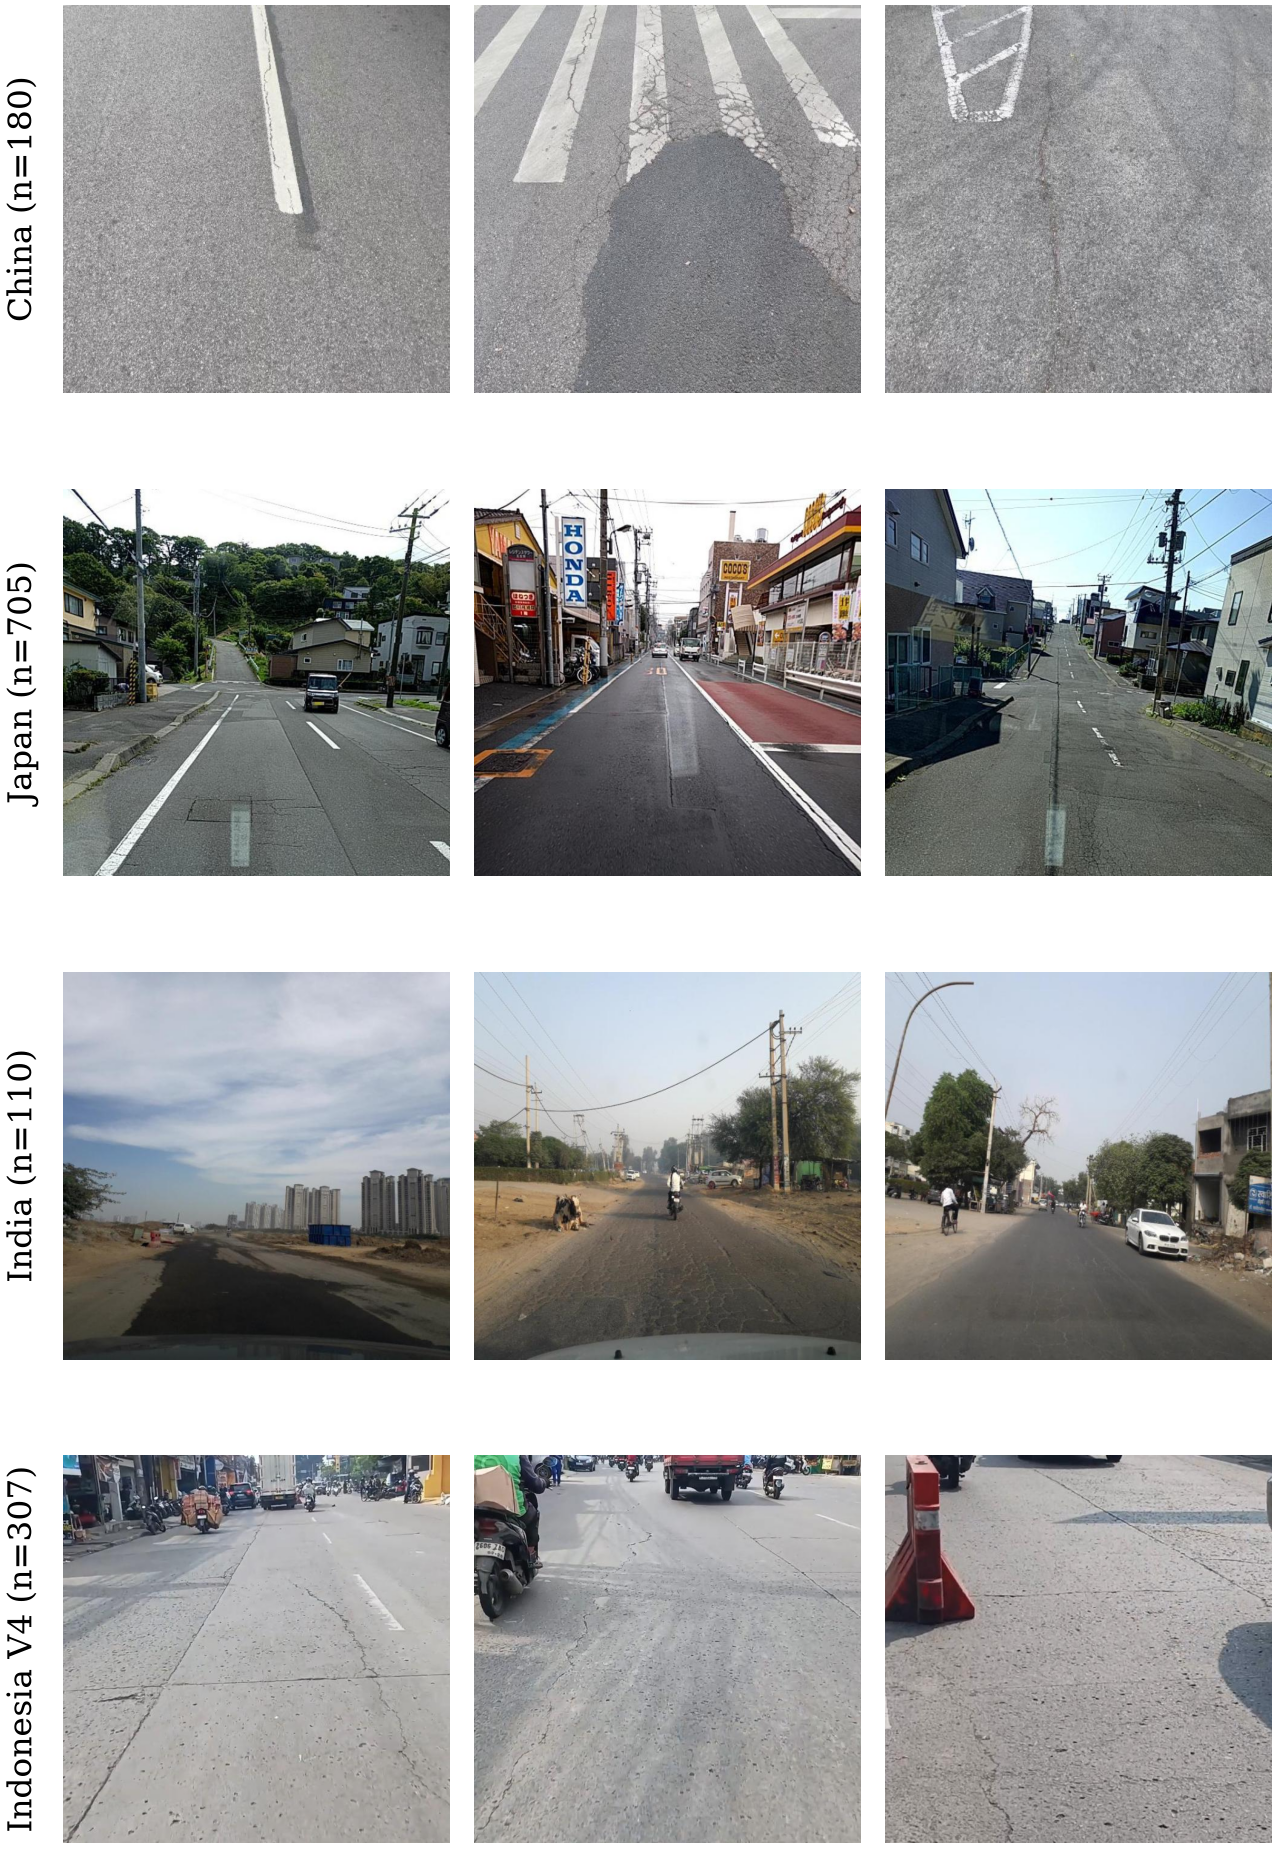
\includegraphics[width=0.68\textwidth]{gambar/paper_figD4_domains.png}
\caption{Three selected images per subset: China (180 test images), Japan (705), India (110), and Indonesia (307 target images). The panels illustrate appearance variation; they are not paired observations of the same scene.}
\label{fig:domain-examples}
\end{figure*}
\fi

\ifdistractoranalysis
% REVIEW-ANALYSIS [provisional]: keep visible in this full-results draft; the
% four-class runs/results are still being finalized before submission.
\subsection{Four- versus Six-Class Training}
Table~\ref{tab:ablation} compares four-class training against six-class training after restricting evaluation of \emph{both} models to the same four damage classes. The four-class runs were higher in mAP@0.5 by 0.0017--0.0108 for three architectures and lower by 0.0008 for YOLO26n. YOLOv8-PD showed the largest observed change (+0.0108). Pothole AP@0.5 increased in each four-class pair, although the change was only about 0.001 for YOLOv12n. Thus, explicit D70/D80 labels did not yield a consistent measured gain for the four principal classes in these runs.

An earlier image-level proxy counted pothole predictions anywhere in images containing D70/D80, even when the prediction did not overlap either object. For YOLOv8n trained on six classes, it counted 53 predictions against 390 distractor ground-truth boxes; a spatial-overlap check found only three. The proxy-based significance tests therefore cannot support a distractor-misclassification claim. Table~\ref{tab:overlap} reports the overlap diagnostic for all four paired architectures. At confidence 0.25 and box IoU at least 0.5, each run yielded only 1--3 pothole predictions overlapping 390 distractor annotations, with none overlapping the 69 patchy-road annotations. The paired differences were zero or one prediction. These counts describe prediction boxes, not uniquely matched objects or a formal false-positive rate. Neither this diagnostic nor the small single-seed AP differences establish a causal benefit from adding D70/D80 labels.

\begin{table}[!htbp]
\centering
\caption{Source test mAP@0.5 over the same four damage classes under each training label set.}
\label{tab:ablation}
\footnotesize
\setlength{\tabcolsep}{4pt}
\begin{tabular}{lrrr}
\toprule
Architecture & Six-class train & Four-class train & Difference \\
\midrule
YOLOv8n   & 0.6224 & 0.6311 & +0.0088 \\
YOLOv12n  & 0.6264 & 0.6280 & +0.0017 \\
YOLO26n   & 0.6044 & 0.6036 & $-0.0008$ \\
YOLOv8-PD & 0.6233 & 0.6341 & +0.0108 \\
\bottomrule
\end{tabular}
\end{table}

\begin{table}[!t]
\centering
\caption{Pothole prediction boxes overlapping distractor ground truth on the source test set (confidence 0.25; overlap IoU $\geq 0.5$; 321 manhole and 69 patchy-road boxes).}
\label{tab:overlap}
\footnotesize
\setlength{\tabcolsep}{4pt}
\begin{tabular}{lrr}
\toprule
Architecture & Six-class train & Four-class train \\
\midrule
YOLOv8n   & 3 & 3 \\
YOLOv12n  & 2 & 3 \\
YOLO26n   & 1 & 2 \\
YOLOv8-PD & 2 & 2 \\
\bottomrule
\end{tabular}
\end{table}
% REVIEW-ANALYSIS [provisional]: overlap is a prediction-box diagnostic,
% not a unique-GT matched-object false-positive rate.
\fi

\subsection{Zero-Shot Target Evaluation}
% REVIEW-ANALYSIS [covered]: Table~\ref{tab:transfer} uses five shared labels;
% Fig.~\ref{fig:class-transfer} shows class-specific AP. The optional
% sensitivity analysis below uses four damage labels on both splits.
Table~\ref{tab:transfer} compares source-test and Indonesian target mAP@0.5 over the same five labels. Every model scored lower on the target export. YOLOv12n had the highest target score (0.337), versus 0.618 on the source test, a 45.5\% relative contrast. YOLO-RD led the five-class source comparison (0.624) but scored 0.302 on the target, below YOLOv12n. The source and target rankings thus differed under this evaluation protocol.

\begin{table}[!htbp]
\centering
\caption{Zero-shot target evaluation vs. source test over the five shared labels (307 target images, 502 instances; no fine-tuning).}
\label{tab:transfer}
\footnotesize
\setlength{\tabcolsep}{3.7pt}
\begin{tabular}{lrrrr}
\toprule
Model & Source mAP & Target mAP & Drop (\%) & Target F1$^{*}$ \\
\midrule
YOLOv8n   & 0.612 & 0.253 & 58.6 & 0.308 \\
YOLOv12n  & 0.618 & \textbf{0.337} & 45.5 & \textbf{0.383} \\
YOLO26n   & 0.586 & 0.249 & 57.5 & 0.281 \\
YOLOv8-PD & 0.611 & 0.286 & 53.3 & 0.312 \\
YOLO-RD   & \textbf{0.624} & 0.302 & 51.6 & 0.336 \\
\bottomrule
\end{tabular}
\par\smallskip
{\scriptsize $^{*}$Macro-F1 over the five target classes with ground truth.\par}
\end{table}

Fig.~\ref{fig:class-transfer} shows that the five-class target contrast was uneven across classes. For YOLOv12n, longitudinal-crack AP@0.5 changed from 0.680 to 0.629 (231 target instances), whereas transverse-crack AP changed from 0.582 to 0.256 (132 instances), pothole from 0.535 to 0.260 (70), and patchy road from 0.587 to 0.036 (21). The low patchy-road score has limited target support. YOLOv12n target macro-F1 was 0.383 versus support-weighted F1 of 0.471; the former gives each of the five classes equal weight. Manhole had no target annotations and was excluded, not scored as zero.

\begin{figure*}[!t]
\centering
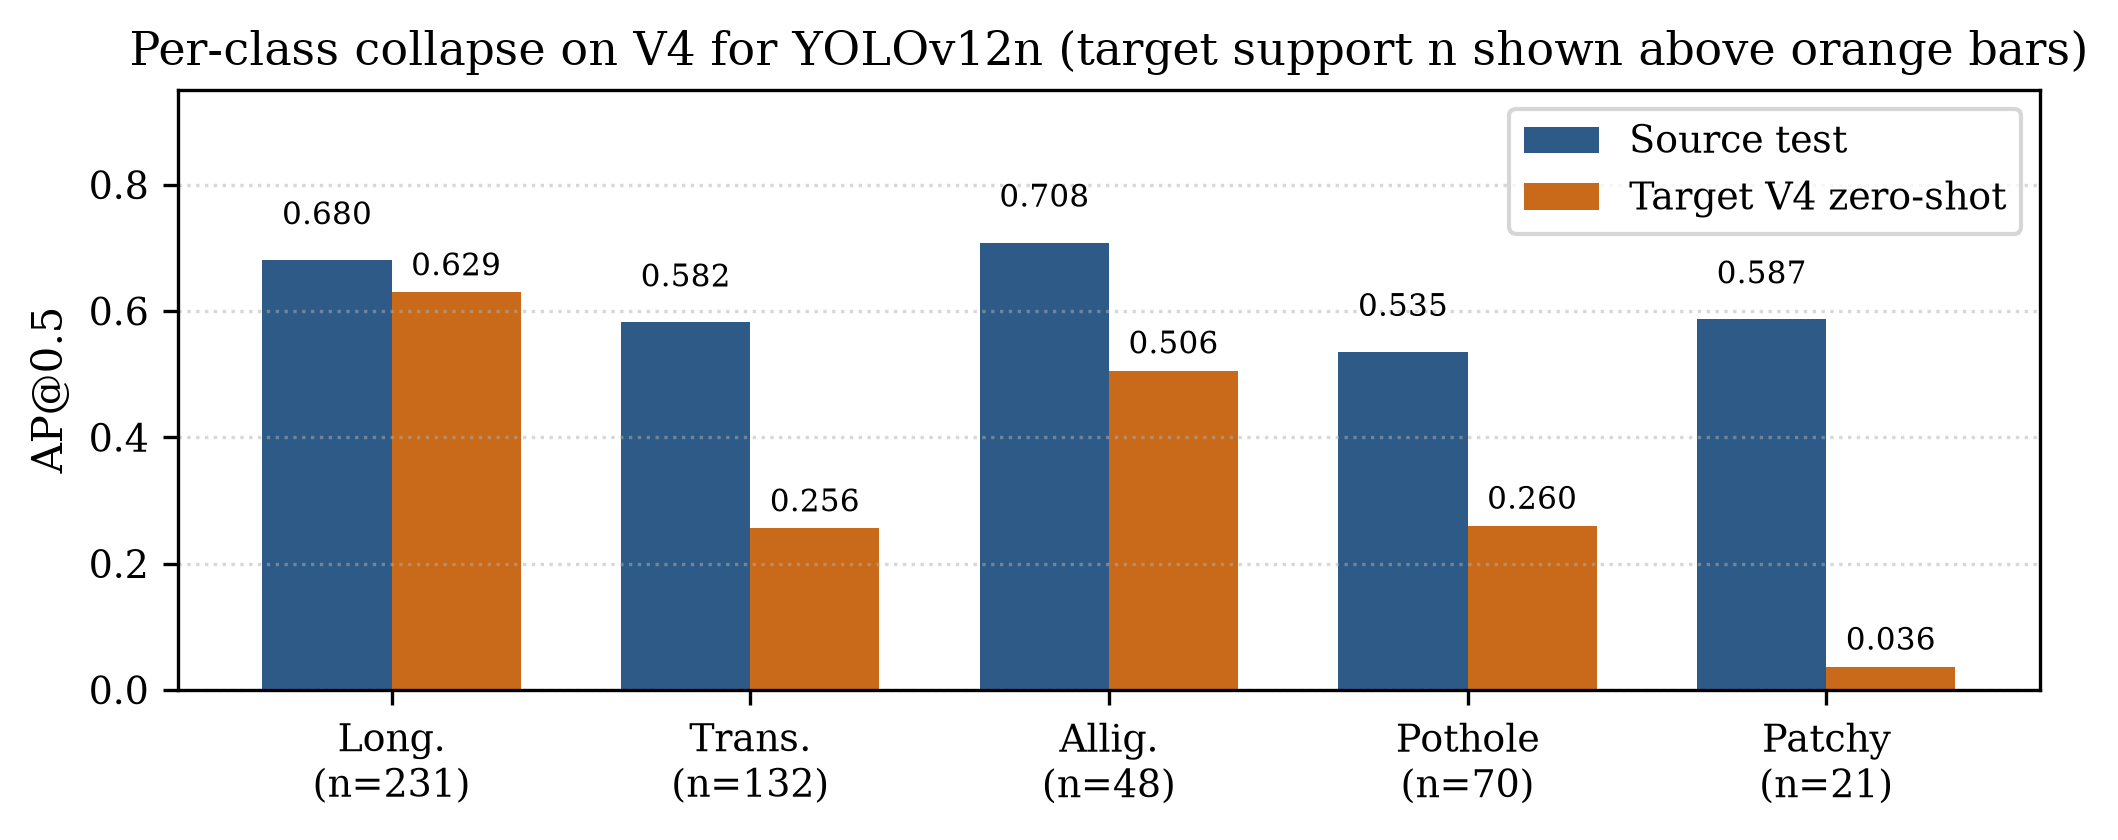
\includegraphics[width=0.82\textwidth]{gambar/paper_fig2_perclass_collapse_v12n.png}
\caption{YOLOv12n AP@0.5 on the source test and Indonesian target export by shared class. Target ground-truth counts appear under class names. The differing test samples limit causal interpretation of the class-specific differences.}
\label{fig:class-transfer}
\end{figure*}

The export differs from the source in data provenance, viewpoints, label support, and sampling. Its lower scores document a cross-set generalization problem under this protocol; they do not identify pavement material, lighting, or geography as a cause. % REVIEW-ANALYSIS [ongoing]: investigate plausible contributors without presenting an untested cause as a finding.

\ifcoretransferanalysis
\subsection{Sensitivity to the Shared Class Set}
The five-class mAP gives patchy road the same weight as each damage class despite its 21 target instances. Table~\ref{tab:core-transfer} repeats the comparison over only the four damage labels on \emph{both} splits. YOLOv12n changed from 0.626 to 0.413, a 34.1\% relative contrast, compared with 45.5\% over five labels. The target performance difference remains under either label set, while the summary's magnitude depends on which classes are averaged.

\begin{table}[!htbp]
\centering
\caption{Source--target mAP@0.5 over only the four shared damage classes.}
\label{tab:core-transfer}
\footnotesize
\setlength{\tabcolsep}{5pt}
\begin{tabular}{lrrr}
\toprule
Model & Source (4) & Target (4) & Drop (\%) \\
\midrule
YOLOv8n   & 0.622 & 0.303 & 51.4 \\
YOLOv12n  & 0.626 & 0.413 & 34.1 \\
YOLO26n   & 0.604 & 0.301 & 50.2 \\
YOLOv8-PD & 0.623 & 0.342 & 45.2 \\
YOLO-RD   & 0.633 & 0.359 & 43.4 \\
\bottomrule
\end{tabular}
\end{table}
\fi

\iffeaturevizanalysis
\subsection{Exploratory Image and Feature Variation}
An earlier visualization used the same 995 source-test images but 308 Indonesian images from a different export. The image-level median brightness was 160.3 in that Indonesian set versus 154.8, 119.4, and 144.0 in China, Japan, and India; a Laplacian-variance sharpness proxy was 532.6 versus 2296.8, 1430.9, and 181.4, respectively. These descriptive summaries depend on camera and scene composition and were not computed on the exact 307-image target export.

A source-trained YOLOv8n embedding of those images is illustrated by the UMAP projection in Fig.~\ref{fig:exploratory-umap}. The plotted groups differ in position, but projection coordinates are arbitrary. Because the target images and annotations do not match the evaluated export exactly, this visualization neither quantifies the reported performance gap nor demonstrates a cause for detection errors.

\begin{figure}[!t]
\centering
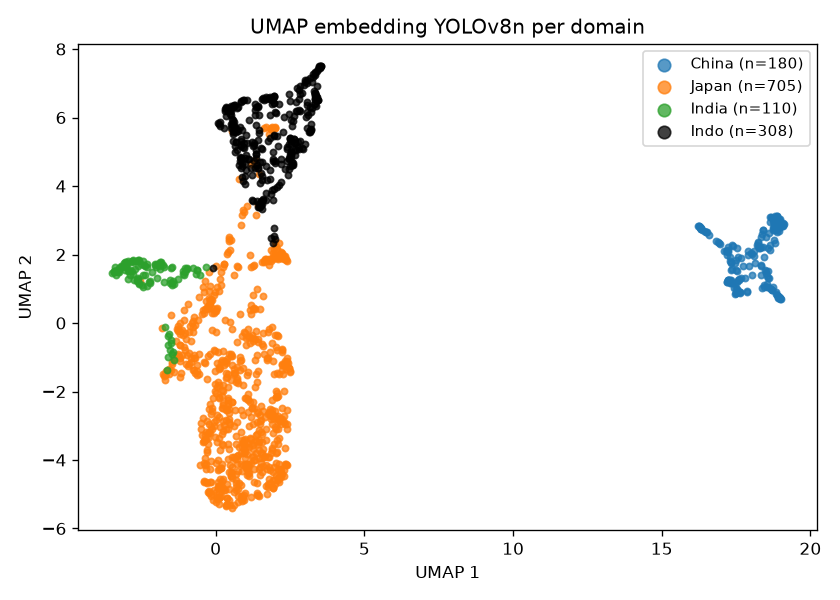
\includegraphics[width=\columnwidth]{gambar/draft_umap_per_domain.png}
\caption{Exploratory YOLOv8n feature UMAP using an earlier 308-image Indonesian export and the 995 source-test images. The target export evaluated in this paper contains 307 images; projection distances are not a physical domain measure.}
\label{fig:exploratory-umap}
\end{figure}
% REVIEW-ANALYSIS [pending]: regenerate descriptive statistics and embedding
% on the frozen 307-image, 502-instance export before using them as direct
% evidence about this evaluation; an older export has 308 images.
\fi

\ifmaterialanalysis
\subsection{Target Error and Correct-Detection Cases}
A selected group of 42 morning-video frames contains 62 target annotations, versus 440 in the other 265 frames. The groups differ in label support: the morning group has no annotated patchy roads and eight potholes, versus 21 and 62, respectively, in the other frames. No matched-class evaluation of these groups was performed; the examples below are illustrative, not an estimate of a glare effect.

Fig.~\ref{fig:target-cases} contrasts two selected target frames with ground truth (GT) and predictions. In the upper morning frame, the annotation file is empty, while YOLOv12n predicts patchy road at confidence 0.78 and YOLOv8-PD predicts pothole at 0.69 on porous-looking pavement. An empty file does not independently verify that every visible feature is defect-free, so this case requires annotation review before a stronger false-positive claim. In the lower frame, all three models identify an annotated longitudinal crack, although the predicted boxes differ. These cases illustrate possible errors and correct detections, not their frequencies or a cause of the aggregate performance difference.

\begin{figure*}[!t]
\centering
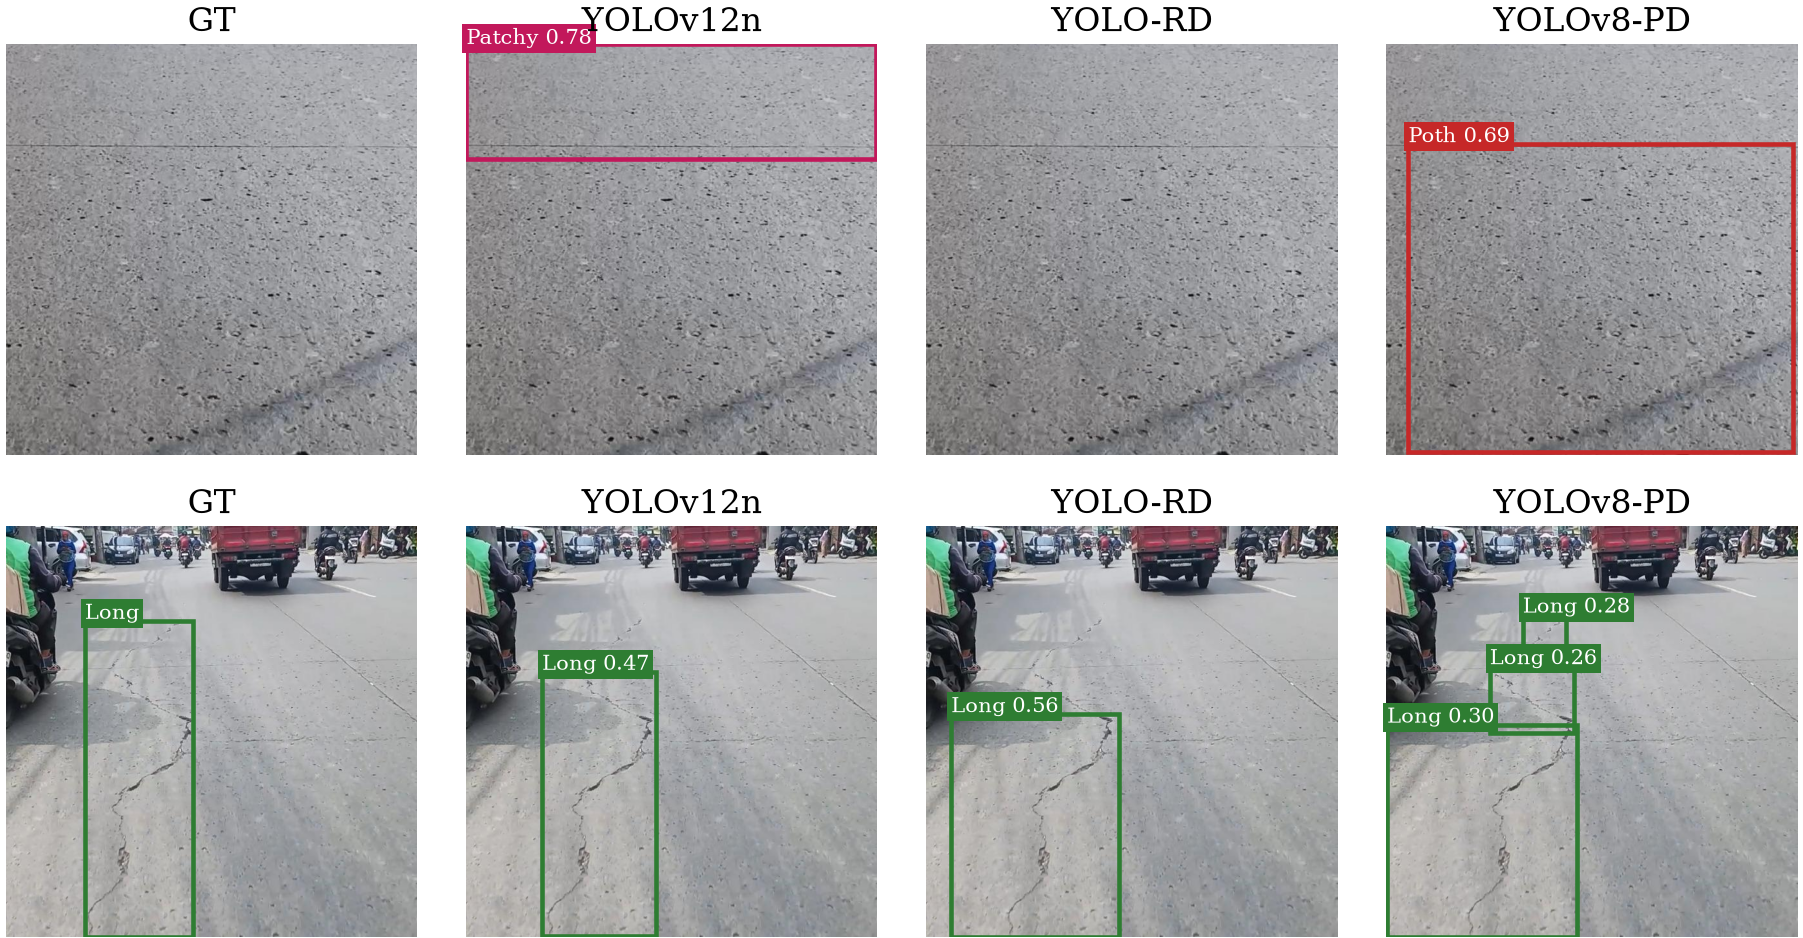
\includegraphics[width=0.86\textwidth]{gambar/paper_figG_error_success_cases.png}
\caption{Two selected Indonesian target frames with GT and predictions from three models at display confidence 0.25: (top) morning porous-looking pavement with an empty annotation file and nonempty predictions; (bottom) an annotated longitudinal crack detected by all three models. Quantitative evaluation uses confidence 0.001.}
\label{fig:target-cases}
\end{figure*}
\fi

\subsection{Limitations}
Each six-class model configuration used a single training seed (42); batch size and mixed-precision settings varied by model. \ifdistractoranalysis Some four-class weights were transferred from a laboratory machine; software-environment equivalence with all six-class runs has not been established. The four-versus-six-class comparison did not include YOLO-RD.\fi{} The local YOLOv8-PD/YOLO-RD reconstructions were not exact author-code replications. Parameter counts and GFLOPs are summary-based complexity estimates rather than device measurements; the throughput protocol needs a canonical timed re-evaluation. The target was an export with only a validation split, not a documented independently sampled test set. A 1080p road-facing smartphone recording and 1-frame/s sampling were reported, but date metadata, frame selection, annotation quality, video-frame dependence, and possible source overlap need further documentation. The current evidence therefore supports descriptive results for this particular target export, not universal claims about deployment in Indonesia.

\section{Conclusion}
In the six-class source evaluation, the local YOLO-RD reconstruction attained the highest mAP@0.5 (0.661), while YOLOv12n attained the highest five-class mAP@0.5 on the zero-shot target export (0.337). \ifdistractoranalysis Comparing the same four damage classes under six- versus four-class training yielded small, mixed changes and did not demonstrate that explicit manhole and patchy-road labels improved damage detection.\fi{} The class-aligned source--target differences motivate evaluation on the intended data before model selection. Multi-seed training, matched-object error analysis, documented target annotation and sampling, and standardized timing are needed before stronger claims about label utility or deployment can be made.

% Balance the bibliography columns on the final page of this full draft.
\IEEEtriggeratref{7}
\bibliographystyle{IEEEtran}
\bibliography{IEEEabrv,references}

\end{document}
